%% paper_template.tex is a modification of:
%% bare_conf.tex 
%% V1.2
%% 2002/11/18
%% by Michael Shell
%% mshell@ece.gatech.edu
%% 
%% This is a skeleton file demonstrating the use of IEEEtran.cls 
%% (requires IEEEtran.cls version 1.6b or later) with an IEEE conference paper.
%% 
%% Support sites:
%% http://www.ieee.org
%% and/or
%% http://www.ctan.org/tex-archive/macros/latex/contrib/supported/IEEEtran/ 
%%
%% This code is offered as-is - no warranty - user assumes all risk.
%% Free to use, distribute and modify.

% *** Authors should verify (and, if needed, correct) their LaTeX system  ***
% *** with the testflow diagnostic prior to trusting their LaTeX platform ***
% *** with production work. IEEE's font choices can trigger bugs that do  ***
% *** not appear when using other class files.                            ***
% Testflow can be obtained at:
% http://www.ctan.org/tex-archive/macros/latex/contrib/supported/IEEEtran/testflow


% Note that the a4paper option is mainly intended so that authors in
% countries using A4 can easily print to A4 and see how their papers will
% look in print. Authors are encouraged to use U.S. letter paper when 
% submitting to IEEE. Use the testflow package mentioned above to verify
% correct handling of both paper sizes by the author's LaTeX system.
%
% Also note that the "draftcls" or "draftclsnofoot", not "draft", option
% should be used if it is desired that the figures are to be displayed in
% draft mode.
%
% This paper can be formatted using the % (instead of conference) mode.
%++++++++++++++++++++++++++++++++++++++++++++++++++++++
%\documentclass[conference]{IEEEims} % Modified for MTT-IMS
%\documentclass[conference]{IMSTemplate}
\documentclass[conference]{IEEEtran}
%++++++++++++++++++++++++++++++++++++++++++++++++++++++
% If the IEEEtran.cls has not been installed into the LaTeX system files, 
% manually specify the path to it:
% \documentclass[conference]{../sty/IEEEtran} 


% some very useful LaTeX packages include:

%\usepackage{cite}      % Written by Donald Arseneau
                        % V1.6 and later of IEEEtran pre-defines the format
                        % of the cite.sty package \cite{} output to follow
                        % that of IEEE. Loading the cite package will
                        % result in citation numbers being automatically
                        % sorted and properly "ranged". i.e.,
                        % [1], [9], [2], [7], [5], [6]
                        % (without using cite.sty)
                        % will become:
                        % [1], [2], [5]--[7], [9] (using cite.sty)
                        % cite.sty's \cite will automatically add leading
                        % space, if needed. Use cite.sty's noadjust option
                        % (cite.sty V3.8 and later) if you want to turn this
                        % off. cite.sty is already installed on most LaTeX
                        % systems. The latest version can be obtained at:
                        % http://www.ctan.org/tex-archive/macros/latex/contrib/supported/cite/

%\usepackage{graphicx}  % Written by David Carlisle and Sebastian Rahtz
                        % Required if you want graphics, photos, etc.
                        % graphicx.sty is already installed on most LaTeX
                        % systems. The latest version and documentation can
                        % be obtained at:
                        % http://www.ctan.org/tex-archive/macros/latex/required/graphics/
                        % Another good source of documentation is "Using
                        % Imported Graphics in LaTeX2e" by Keith Reckdahl
                        % which can be found as esplatex.ps and epslatex.pdf
                        % at: http://www.ctan.org/tex-archive/info/
% NOTE: for dual use with latex and pdflatex, instead load graphicx like:
%\ifx\pdfoutput\undefined
%\usepackage{graphicx}
%\else
%\usepackage[pdftex]{graphicx}
%\fi
%+++++++++++++++++++++++++++++++++++++++++++
% Added to commands
\input epsf
\usepackage{graphicx}
\usepackage[portuguese]{babel}
\usepackage[utf8x]{inputenc}
\usepackage{listings}
%+++++++++++++++++++++++++++++++++++++++++++
% However, be warned that pdflatex will require graphics to be in PDF
% (not EPS) format and will preclude the use of PostScript based LaTeX
% packages such as psfrag.sty and pstricks.sty. IEEE conferences typically
% allow PDF graphics (and hence pdfLaTeX). However, IEEE journals do not
% (yet) allow image formats other than EPS or TIFF. Therefore, authors of
% journal papers should use traditional LaTeX with EPS graphics.
%
% The path(s) to the graphics files can also be declared: e.g.,
% \graphicspath{{../eps/}{../ps/}}
% if the graphics files are not located in the same directory as the
% .tex file. This can be done in each branch of the conditional above
% (after graphicx is loaded) to handle the EPS and PDF cases separately.
% In this way, full path information will not have to be specified in
% each \includegraphics command.
%
% Note that, when switching from latex to pdflatex and vice-versa, the new
% compiler will have to be run twice to clear some warnings.


%\usepackage{psfrag}    % Written by Craig Barratt, Michael C. Grant,
                        % and David Carlisle
                        % This package allows you to substitute LaTeX
                        % commands for text in imported EPS graphic files.
                        % In this way, LaTeX symbols can be placed into
                        % graphics that have been generated by other
                        % applications. You must use latex->dvips->ps2pdf
                        % workflow (not direct pdf output from pdflatex) if
                        % you wish to use this capability because it works
                        % via some PostScript tricks. Alternatively, the
                        % graphics could be processed as separate files via
                        % psfrag and dvips, then converted to PDF for
                        % inclusion in the main file which uses pdflatex.
                        % Docs are in "The PSfrag System" by Michael C. Grant
                        % and David Carlisle. There is also some information 
                        % about using psfrag in "Using Imported Graphics in
                        % LaTeX2e" by Keith Reckdahl which documents the
                        % graphicx package (see above). The psfrag package
                        % and documentation can be obtained at:
                        % http://www.ctan.org/tex-archive/macros/latex/contrib/supported/psfrag/

%\usepackage{subfigure} % Written by Steven Douglas Cochran
                        % This package makes it easy to put subfigures
                        % in your figures. i.e., "figure 1a and 1b"
                        % Docs are in "Using Imported Graphics in LaTeX2e"
                        % by Keith Reckdahl which also documents the graphicx
                        % package (see above). subfigure.sty is already
                        % installed on most LaTeX systems. The latest version
                        % and documentation can be obtained at:
                        % http://www.ctan.org/tex-archive/macros/latex/contrib/supported/subfigure/

%\usepackage{url}       % Written by Donald Arseneau
                        % Provides better support for handling and breaking
                        % URLs. url.sty is already installed on most LaTeX
                        % systems. The latest version can be obtained at:
                        % http://www.ctan.org/tex-archive/macros/latex/contrib/other/misc/
                        % Read the url.sty source comments for usage information.

%\usepackage{stfloats}  % Written by Sigitas Tolusis
                        % Gives LaTeX2e the ability to do double column
                        % floats at the bottom of the page as well as the top.
                        % (e.g., "\begin{figure*}[!b]" is not normally
                        % possible in LaTeX2e). This is an invasive package
                        % which rewrites many portions of the LaTeX2e output
                        % routines. It may not work with other packages that
                        % modify the LaTeX2e output routine and/or with other
                        % versions of LaTeX. The latest version and
                        % documentation can be obtained at:
                        % http://www.ctan.org/tex-archive/macros/latex/contrib/supported/sttools/
                        % Documentation is contained in the stfloats.sty
                        % comments as well as in the presfull.pdf file.
                        % Do not use the stfloats baselinefloat ability as
                        % IEEE does not allow \baselineskip to stretch.
                        % Authors submitting work to the IEEE should note
                        % that IEEE rarely uses double column equations and
                        % that authors should try to avoid such use.
                        % Do not be tempted to use the cuted.sty or
                        % midfloat.sty package (by the same author) as IEEE
                        % does not format its papers in such ways.

%\usepackage{amsmath}   % From the American Mathematical Society
                        % A popular package that provides many helpful commands
                        % for dealing with mathematics. Note that the AMSmath
                        % package sets \interdisplaylinepenalty to 10000 thus
                        % preventing page breaks from occurring within multiline
                        % equations. Use:
%\interdisplaylinepenalty=2500
                        % after loading amsmath to restore such page breaks
                        % as IEEEtran.cls normally does. amsmath.sty is already
                        % installed on most LaTeX systems. The latest version
                        % and documentation can be obtained at:
                        % http://www.ctan.org/tex-archive/macros/latex/required/amslatex/math/



% Other popular packages for formatting tables and equations include:

%\usepackage{array}
% Frank Mittelbach's and David Carlisle's array.sty which improves the
% LaTeX2e array and tabular environments to provide better appearances and
% additional user controls. array.sty is already installed on most systems.
% The latest version and documentation can be obtained at:
% http://www.ctan.org/tex-archive/macros/latex/required/tools/

% Mark Wooding's extremely powerful MDW tools, especially mdwmath.sty and
% mdwtab.sty which are used to format equations and tables, respectively.
% The MDWtools set is already installed on most LaTeX systems. The lastest
% version and documentation is available at:
% http://www.ctan.org/tex-archive/macros/latex/contrib/supported/mdwtools/


% V1.6 of IEEEtran contains the IEEEeqnarray family of commands that can
% be used to generate multiline equations as well as matrices, tables, etc.


% Also of notable interest:

% Scott Pakin's eqparbox package for creating (automatically sized) equal
% width boxes. Available:
% http://www.ctan.org/tex-archive/macros/latex/contrib/supported/eqparbox/



% Notes on hyperref:
% IEEEtran.cls attempts to be compliant with the hyperref package, written
% by Heiko Oberdiek and Sebastian Rahtz, which provides hyperlinks within
% a document as well as an index for PDF files (produced via pdflatex).
% However, it is a tad difficult to properly interface LaTeX classes and
% packages with this (necessarily) complex and invasive package. It is
% recommended that hyperref not be used for work that is to be submitted
% to the IEEE. Users who wish to use hyperref *must* ensure that their
% hyperref version is 6.72u or later *and* IEEEtran.cls is version 1.6b 
% or later. The latest version of hyperref can be obtained at:
%
% http://www.ctan.org/tex-archive/macros/latex/contrib/supported/hyperref/
%
% Also, be aware that cite.sty (as of version 3.9, 11/2001) and hyperref.sty
% (as of version 6.72t, 2002/07/25) do not work optimally together.
% To mediate the differences between these two packages, IEEEtran.cls, as
% of v1.6b, predefines a command that fools hyperref into thinking that
% the natbib package is being used - causing it not to modify the existing
% citation commands, and allowing cite.sty to operate as normal. However,
% as a result, citation numbers will not be hyperlinked. Another side effect
% of this approach is that the natbib.sty package will not properly load
% under IEEEtran.cls. However, current versions of natbib are not capable
% of compressing and sorting citation numbers in IEEE's style - so this
% should not be an issue. If, for some strange reason, the user wants to
% load natbib.sty under IEEEtran.cls, the following code must be placed
% before natbib.sty can be loaded:
%
% \makeatletter
% \let\NAT@parse\undefined
% \makeatother
%
% Hyperref should be loaded differently depending on whether pdflatex
% or traditional latex is being used:
%
%\ifx\pdfoutput\undefined
%\usepackage[hypertex]{hyperref}
%\else
%\usepackage[pdftex,hypertexnames=false]{hyperref}
%\fi
%
% Pdflatex produces superior hyperref results and is the recommended
% compiler for such use.



% *** Do not adjust lengths that control margins, column widths, etc. ***
% *** Do not use packages that alter fonts (such as pslatex).         ***
% There should be no need to do such things with IEEEtran.cls V1.6 and later.


% correct bad hyphenation here
\hyphenation{agile-modelling eXtreme-programming feature-driven model-driven just-in-time}
\begin{document}

% paper title
%\title{Submission Format for IMS2014 (Title in 24-point Times font)}
% If the \LARGE is deleted, the title font defaults to  24-point.
% Actually, 
% the \LARGE sets the title at 17 pt, which is close enough to 18-point.
%+++++++++++++++++++++++++++++++++++++++++++
\title{\LARGE Estudo Simples sobre Agile Modeling (AM)}
%+++++++++++++++++++++++++++++++++++++++++++
% author names and affiliations
% use a multiple column layout for up to three different
% affiliations
%+++++++++++++++++++++++++++++++++++++++++++
%\author{\authorblockN{J. Clerk Maxwell}
%\authorblockA{School of Electrical and\\Computer Engineering\\
%Somewhere Institute of Technology\\
%City, State 54321--0000\\
%Email: maxwell@curl.edu}
%\and
%\authorblockN{Michael Faraday}
%\authorblockA{(List authors on this line using 12 point Times font\\ - use a second line if necessary)\\
%Microwave Research\\
%City, State/Region, Mail/Zip Code, Country\\
%Email: homer@thesimpsons.com}
%\and
%\authorblockN{Andr\'e M. Amp\`ere \\ }
%\authorblockA{Starfleet Academy\\
%San Francisco, CA 96678-2391\\
%Telephone: (800) 555--1212\\
%Fax: (888) 555--1212}}

\author{
  \authorblockN{
    Lucas P. Tonussi
    \authorrefmark{1}
    \authorblockA{
      \authorrefmark{1}
      Departamento de Informática e Estatística\\
      Universidade Federal de Santa Catarina\\
      tonussi@inf.ufsc.br\\
    }
  }
}

%+++++++++++++++++++++++++++++++++++++++++++++++++++

% avoiding spaces at the end of the author lines is not a problem with
% conference papers because we don't use \thanks or \IEEEmembership


% for over three affiliations, or if they all won't fit within the width
% of the page, use this alternative format:
% 
% Another example.
%\author{\authorblockN{Michael Shell\authorrefmark{1},
%Homer Simpson\authorrefmark{2},
%James Kirk\authorrefmark{3}, 
%Montgomery Scott\authorrefmark{3} and
%Eldon Tyrell\authorrefmark{4}}
%\authorblockA{\authorrefmark{1}School of Electrical and Computer Engineering\\
%Georgia Institute of Technology,
%Atlanta, Georgia 30332--0250\\ Email: mshell@ece.gatech.edu}
%\authorblockA{\authorrefmark{2}Twentieth Century Fox, Springfield, USA\\
%Email: homer@thesimpsons.com}
%\authorblockA{\authorrefmark{3}Starfleet Academy, San Francisco, California 96678-2391\\
%Telephone: (800) 555--1212, Fax: (888) 555--1212}
%\authorblockA{\authorrefmark{4}Tyrell Inc., 123 Replicant Street, Los Angeles, California 90210--4321}}



% use only for invited papers
%\specialpapernotice{(Invited Paper)}

% make the title area
\maketitle

\begin{abstract}
Minha abordagem princípal é entender melhor o desenvolvimento ágil, estudando mais aprofundadamente a modelagem ágil.
\end{abstract}
\IEEEoverridecommandlockouts
\begin{keywords}
Agile, software development model, agile modeling, agile documentation.
\end{keywords}
% no keywords

% For peer review papers, you can put extra information on the cover
% page as needed:
% \begin{center} \bfseries EDICS Category: 3-BBND \end{center}
%
% for peerreview papers, inserts a page break and creates the second title.
% Will be ignored for other modes.
\IEEEpeerreviewmaketitle


\section{Introdução}
% no \PARstart
Modelagem ágil (Agile Modeling - AM) deve ser entendida como um complemento à métodos. Métodos de desenvolvimento de software, esses, podendo ser por exemplo RUP, Unified Process, XP eXtreme Programming, SCRUM, dentre outros. Assim a busca nesse artigo é tentar entender, desmistificar a modelagem ágil baseando-se no livro do Scott Ambler\cite{scott}.

\section{Visão Princípal}
Modelagem Ágil (AM - Agile Modeling) é uma prática para {\bfseries modelagem e documentação} efetiva (ou seja não necessáriamente ágil significa documentação de lado e produção a todo vapor). AM é um método que visa, desenvolvimento e projeto de software como sistema. Agile Modeling (AM) é uma coleção de valores, princípios e práticas. Para modelagem de software que pode ser aplicada no desenvolvimento de um projeto de software de maneira simples e efetiva.

Os valores da modelagem ágil, adotam e exportam do eXtreme Programming, que são: {\bfseries comunicação, retorno (feedback), coragem, e humildade}. O objetivo é que você tenha comunicação efetiva. Como por exemplo telefones sempre a mão dos analístas de sistema, engenheiros de usabilidade, e até mesmo dos programadores, para que eles possam acionar rapidamente o cliente, ou a equipe. Se o cliente, então para poder desvendar alguma história de usuário (se você estiver trabalhando com SCRUM) ou ainda CRC Cards (SCRUM ou eXtreme Programming ou FDD). A comunicação deve ser eficiente, rápida entre todos os stakeholders do projeto em ação. O motivo, obter feedback mantendo o resultado do esforço da equipe, constante durante o começo do projeto, que é onde muitas desmistificações acontecem. E também onde riscos do projeto são entendídas. Para ter a coragem de fazer e ter certeza de suas decisões, e também ter a humildade para admitir que você pode não saber tudo. Que outros tem valor para adicionar melhorias ao seu eforço em cima do projeto. Ou ainda, criticar o seu trabalho (esforço aplicado no projeto).

\section{Princípios}
AM é baseado numa coleção de princípios, tais como assumir simplicidade quando você está modelando e {\bfseries abraçar a mudança} conforme você está trabalhando, por causa que os requerimentos irão mudar com o passar dos ciclos iterativos. Você deveria reconhecer/aceitar que o variação incremental do seu sistema pelo tempo possibilita agilidade e que você deveria almejar em obter rápido retorno (feedback) no seu trabalho para se assegurar que isso reflete com precisão as necessidades do stackholders do projeto. Você deveria modelar com propósito, pois se você não sabe a razão pela qual você está produzindo esse artefato (modelo/documento) então você pode estár gastando esforços em algo desnecessário. Lembremos que a equipe deverá trabalhar junta, isso que dizer que usando de coragem (princípio) você aponta para a possibilidade de modelar/documentar artefatos $Art_1, Art_2, ...,Art_n$ então na reunião com a equipe, proponha isso e alguma sugestão, alguma retorno vai ter isso. Pior é se você não participar executando os princípios e práticas daquele método de desenvolvimento que a empresa custuma adotar para a construção de software e administração da equipe. Um conceito crítico é que modelos não são necessariamente documentos. Uma realização que possibilita que você se organize melhor, desempenhe melhor no seu trabalho, como analísta ou desenvolvedor, descartando a maioria de seus modelos uma vez que eles cumpriram sua missão. Modeladores ágeis acreditam que conteúdo é mais importânte que representação, que existem muitos caminhos para você modelar a mesma coisa, da maneira que a equipe vai pegar a ideia. Para ser um modelador de efeito, você precisa reconhecer que ser {\bfseries aberto e honesto} na sua comunicação é comumente a melhor política a ser seguida, para asegurar eficássia. Finalmente foco em trabalho qualificado (eXtreme Programming por exemplo aponta que Pair Programming é muito eficaz pois o código sai 1: testado 2: revisado) é importante pois o gerênte de projeto e a equipe também não irão gostar de trabalho desqualificado, fora do padrão. Não dá para ficar arriscando quando se trata de competição no mercado de software. Adaptação é ponto vital (importânte) na modelagem ágil, isso permite abordar necessidades inusitádas vindas de dentro do ambiente (Bibliotecas melhores, Tecnologia diferente) ou externamente ao ambiente (Cliente).

\section{Work Item List: Disciplined Agile}
A abordagem da figura ~\ref{fig:workitens} reflete o que se espera de uma construção ágil disciplinada de fila de Work Items. Essa técnica é explicada pela Entregas Ágeis Disciplinadas (Disciplined Agile Delivery - DAD). As vantagens da Lista de Work Items são que facilmente suportam diferenças nas iterações, ou seja tipos diferentes de Work Items. E "Overhead fudge factor" (Fudge factor é um hack para fazer com que um modelo qualquer se encaixe nas expectativas) requerido é muito menor ou não existente se comparado com a abordagem do SCRUM de product backlog. As desvantagens são: Ter que mander Work Items da fila priorizados paralelamente com prioridades sendo alteradas durante o decorrer da iteração. Requer múltiplas filas de Work Items, ou um esquema de priorização mais complexo, para suportar Classes of Service.

\subsection{Classes de Serviço}
David J. Anderson categoriza trabalho por risco e tipo e então associa isso com uma classe de serviço específica como: Classes para Work Items que irão salvar tempo no cronograma, classes para Work Items que violam copyright, classes com prioridade para Work Items de maior risco para o sistema. Ou seja a ideia é nenhum Work Item deveria ser tratado igual. Isso permite aos programadores entregar software com risco controlado, gerando maior fluxo de trabalho, e aumentando previsão do produto a cada iteração\cite{dpjoyce}.

\subsection{Valores dos Riscos}
De valor aos riscos. Sobre isso podemos incluir o risco de precisar chegar a uma conclusão com os stakeholders o mais cedo possível do projeto. O risco pode ser melhor entendído se a equipe tem visão ampla e melhor ainda se os engenheiros estão acostumados com método ágil. Outro risco que podemos ligar é o risco de provar que a sua visão de arquitetura funciona. Como mostrar para o Cliente que funciona ? O jeito bastante bom é codificar uma arquitetura esqueleto. Desenvolvedores espertos irão olhar para os Work Items da fila, no começo do projeto e identificar riscos nos requisitos para já tentar criar alternativas para resolve-los já logo no primeiro Sprint. Caso o requisito risco, que foi identificado não está em cima da fila para ser resolvido primeiro ? Convoca uma reunião e mostra o por que daquele Work Item deveria estár na frente da fila, naturalmente que os desenvolvedores, analístas e stakeholders irão chegar a um "concensus".

\subsection{Modele um pouco a frente}
É bom muitas vezes para quando a fila for sendo esvaziada de Work Items, os próximos requisitos vão sendo mais fáceis de desmistificar. Se um Work Item é muito complexo vale a pena investir mais tempo nele, usando uma técnica chamada Look-Ahead também usando no SCRUM, mas com o nome de Backlog Grooming. Basicamente é você olhar para 2~3 Work Itens a frente e entender como aquele Work Item atual é complexo, o quanto ele é. Onde ele afeta ou não o sistema. Nisso você está trabalhando ágilmente sobre riscos. A figura ~\ref{fig:workitens} ilustra como a fila de Work Items funciona.

\begin{figure}[ht]
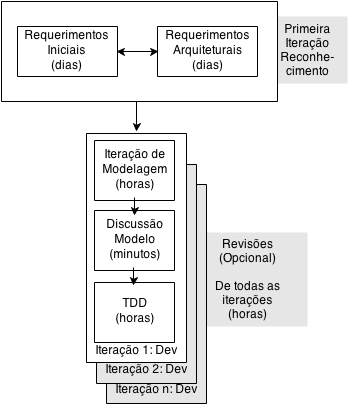
\includegraphics[scale=0.65]{amdd.png}
%\epsfxsize=3.25in\epsfbox{figure1.epsi}
\caption{Esquematização do funcionamento básico de manipulação de "Working Itens".}
\label{fig:workitens}
\end{figure}

\section{Práticas}
Para modelar no espírito Ágil você deverá aplicar práticas ágeis de modelagem. Práticas fundamentais incluem criar modelagens em paralelo, aplicando os artefatos corretamente para cada situação, interagir em outros artefatos para continuar movendo eles para frente até um estado aceitável, regular também é válido. Modelar em pequenos incrementos, conforme a necessidade é mais aceitável do que criar modelagens massivas de uma vez só, o que não tem boa aceitação. Até porque a equipe gostaria de escalar todos juntos, ao invéz de um faz a escalada sozinho, chega no topo e fica esperando a equipe nivelar com ele novamente.

\subsection{Representações Abstratas}
Modelos são apenas representações abstratas de software, abstrações que podem não ser precisar, você deveria buscar provar que seu {\bfseries código} funciona como você o tinha idealizado anteriormente. Isso não tem mistério uma vez que você estuda TDD e não deixa o TDD apenas na teoria, mas se força a aplicar TDD, justamente para provar o que você construiu. Participação dos stakeholders é imprecindível para que a equipe tenha esforço gerando sucesso com as modelagens. Simplesmente por que os stakeholders do projeto sabem o que eles querem, e eles podem te retornar explicações do que eles querem. O princípio de assumir simplicidade é suportado pela prática de criar conteúdo simples, focando apenas no aspecto que você precisa para modelar e não tentar criar um extremamente super modelo detalhado.

\subsection{Configuração da Comunicação}
Comunicação atravéz de mural que mostra os modelos publicamente, atravéz de um website apenas para mostrar publicamente, como linha do tempo o que se tem feito, onde a equipe está, o que se planeja. Um exemplo é o Redmine que é uma ferramenta gratuíta e aberta, de administração de projeto e ferramenta de perseguição de falhar no produto. Inclue calendário e diagramas Gantt que visam ajudar com representações visuais do projeto e suas deadlines.

\section{TDD e Agile Modeling}
O primeiro passo é entender o TFD, Test First Development onde você adiciona rapidamente um test, e testa se ele passar você adiciona mais testes, se ele falhar você adiciona uma pequena mudança (note que a meta é adicionar teste que falha). E então roda os testes novamente, se falhar então mais uma pequena mudança e fica nesse ciclo até não falhar mais, e então se passarem. Você volta ao início e adiciona mais testes novos. {\bfseries Sempre pensando em adicionar aos poucos. E modificar aos poucos.} Assim você tem entendimento do que você está fazendo. Com prática você irá programar mais rápido do que sair direto jogando código funcional. O ciclo do TFD acaba quando você voltou ao início dessa atividade e reconheceu que você terminou de implementar o que precisava. O TDD entra aqui. Quando você tem feito TFD e Refatorado. Essas operações juntas são o TDD sendo aplicado. Porém o TDD vai um pouco mais fundo, existem atividades de ATDD. ATDD é aceitação do TDD. É uma atividade que engloba o TFD. Onde você roda testes de aceitação para os seus testes de funcionalidade. Muitos programadores ignoram ATDD. Pois hoje em dia os Frameworks de Test, auxiliam muito nessa parte. Tecnologias que você pode estár abordando são: para ATDD RSpec, Fitnesse e para Agile TDD programadores poderão usar xUnit Frameworks. No site: http://agiledata.org você poderá encontrar mais sobre TDD e outras formas de desenvolvimento dirigido a testes, você poderá descobrir também que existem formas de modelagem de banco de dados e testes de transações com banco de dados tudo dirigido a testes.

\subsection{Scalando TDD via Agile Model-Driven Development (AMDD)}
TDD é uma ferramenta de especificação e validação. Mas não pensemos em usar TDD apenas sob grandes problemas de design, mas também como as pessoas irão usar o sistema (engenharia de usabilidade). Ou por exemplo: na interface de usuário. Modelar ou sendo mais específico utilizar Agile model-driven development (AMDD) junto com TDD para completar problemas como escalabilidade ágil, mas o AMDD implementa escalabilidade ágil (veja figura ~\ref{fig:requirements}).

\section{Requisitos}
Poderiamos dizer que o AM é uma medida ágil para modelagem, que o núcleo do AM é simplesmente uma coleção de práticas que refletem os princípios e valores que foram construídos por desenvolvedores de software muito experiêntes, que viram a necessidade de publicar isso. Com o Modelo de Desenvolvimento Ágil Dirigido (Agile Model Driven Development - veja figura 2 ~\ref{fig:requirements}). A abordagem é aplicar modelagem alto-nível no começo do projeto para entender o escopo e o potencial da arquitetura. E então durante o desenvolvimento das iterações você modela as partes da sua iteração planejando atividades e então aplica modelagem just-in-time (JIT) (na forma de "brain storming") onde você modela por muitos minutos antes de ficar por muitas horas codificando. Vamos entender essa imagem ~\ref{fig:requirements}). No primeiro retângulo superior o que precisa ser entendido é que a equipe deveria: Identificar o escopo de alto-nível. Identificar a pilha de requisitos do sistema (iniciais). E identificar a visão arquitetural. Logo abaixo ao retângulo superior vemos as iterações de desenvolvimento onde deveríamos entender: Que modelagem é parte do esforço iterativo, modelar o suficiente para ter boas estimativas. É como se você estivesse em uma Rally. Você é o motorista e irá dirigir atravéz das iterações. E existe um navegador que entende o percurso para o piloto. Essa filosofia de fazer o caminho dando passos pensados é bastante a cara do método ágil. Você precisa também planejar o trabalho da equipe para aquela iteração (naturalmente). Trabalhar atravéz de problemas usando JIT. Stakeholders como participantes ativos do processo. Requisitos do sistema, evoluem com o desenrolar do projeto. Modelo o suficiênte para o momento, você poderá voltar e re-modelar depois. Construa software via através de test-first.

\begin{figure}[ht]
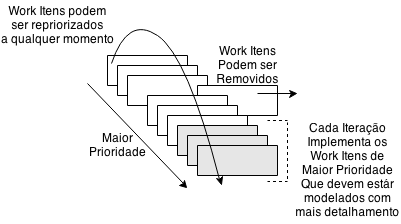
\includegraphics[scale=0.55]{requirements.png}
%\epsfxsize=3.25in\epsfbox{figure1.epsi}
\caption{Esquematização do funcionamento básico de manipulação de "Working Itens".}
\label{fig:requirements}
\end{figure}

Os valores da modelagem ágil, adotam e exportam do eXtreme Programming, que são: {\bfseries comunicação, retorno (feedback), coragem, e humildade}. O objetivo é que você tenha comunicação efetiva. Como por exemplo telefones sempre a mão dos analístas de sistema, engenheiros de usabilidade, e até mesmo dos programadores, para que eles possam acionar rapidamente o cliente, ou a equipe. Se o cliente, então para poder desvendar alguma história de usuário (se você estiver trabalhando com SCRUM) ou ainda CRTCards (SCRUM ou eXtreme Programming ou FDD). A comunicação deve ser eficiente, rápida entre todos os stakeholders do projeto em ação. O motivo, obter feedback mantendo o resultado do esforço da equipe, constante durante o começo do projeto, que é onde muitas desmistificações acontecem. E também onde riscos do projeto são entendídas. Para ter a coragem de fazer e ter certeza de suas decisões, e também ter a humildade para admitir que você pode não saber tudo. Que outros tem valor para adicionar melhorias ao seu eforço em cima do projeto. Ou ainda, criticar o seu trabalho (esforço aplicado no projeto).

% The following statement makes the two columns on the last page more
% or less of equal length.  Placement of this command is by trial and error.
\vfil\eject

% Reminder: the "draftcls" or "draftclsnofoot", not "draft", class option
% should be used if it is desired that the figures are to be displayed while
% in draft mode.

% An example of a floating figure using the graphicx package.
% Note that \label must occur AFTER (or within) \caption.
% For figures, \caption should occur after the \includegraphics.
%
%\begin{figure}
%\centering
%\includegraphics[width=2.5in]{myfigure}
% where an .eps filename suffix will be assumed under latex, 
% and a .pdf suffix will be assumed for pdflatex
%\caption{Simulation Results}
%\label{fig_sim}
%\end{figure}

% An example of a double column floating figure using two subfigures.
%(The subfigure.sty package must be loaded for this to work.)
% The subfigure \label commands are set within each subfigure command, the
% \label for the overall fgure must come after \caption.
% \hfil must be used as a separator to get equal spacing
%
%\begin{figure*}
%\centerline{\subfigure[Case I]{\includegraphics[width=2.5in]{subfigcase1}
% where an .eps filename suffix will be assumed under latex, 
% and a .pdf suffix will be assumed for pdflatex
%\label{fig_first_case}}
%\hfil
%\subfigure[Case II]{\includegraphics[width=2.5in]{subfigcase2}
% where an .eps filename suffix will be assumed under latex, 
% and a .pdf suffix will be assumed for pdflatex
%\label{fig_second_case}}}
%\caption{Simulation results}
%\label{fig_sim}
%\end{figure*}

% An example of a floating table. Note that, for IEEE style tables, the 
% \caption command should come BEFORE the table. Table text will default to
% \footnotesize as IEEE normally uses this smaller font for tables.
% The \label must come after \caption as always.
%
%\begin{table}
%% increase table row spacing, adjust to taste
%\renewcommand{\arraystretch}{1.3}
%\caption{An Example of a Table}
%\label{table_example}
%\begin{center}
%% Some packages, such as MDW tools, offer better commands for making tables
%% than the plain LaTeX2e tabular which is used here.
%\begin{tabular}{|c||c|}
%\hline
%One & Two\\
%\hline
%Three & Four\\
%\hline
%\end{tabular}
%\end{center}
%\end{table}
%\begin{table}
%\caption{An Example of a Table}
%\label{table_example}
%\begin{center}
%\begin{tabular}{|c||c|}
%\hline
%One & Two\\
%\hline
%Three & Four\\
%\hline
%\end{tabular}
%\end{center}
%\end{table}

\section{Conclusão}
A modelagem ágil deve ser agregada a outros métodos de desenvolvimento. Deve-se entender que Agile Modeling não é para equipes grandes. E principalmente não vai ser aplicada a equipes sem experiência. Equipes maiores que 30 pessoas, é um risco a ser tomado. Equipes com analístas e programadores com menos de 2 anos de experiência, é outro risco a ser tomado. Programadores que não executaram projetos utilizando métodos ágeis, anteriormente na sua carreira, é mais um risco a ser tomado. O autor observa a possibilidade de integrar AM com eXtreme Programming. Eu particularmente, conhecendo XP, não vejo como. Mas todavia eu entendo um pouco a sugestão dele, que é de quando você tem uma equipe experiênte que se adapata ao XP mas eles precisam utilizar em alguns projetos boas quantidades de modelagem. Então Modele utilizando os princípios do AM pois você não irá perder nada com isso, você vai estár dentro do método ágil. Agora UP e AM eu vejo como eles poderiam se unir pois UP é bastante flexível e UP aborda a idéia de que software deve ser entregue iterativamente e incrementalmente que é a mesma idéia de AM. E UP aborda explícitamente disciplinas de modelagem e é simples em identificar onde as práticas do AM poderiam ser usadas para melhorar o UP.

% conference papers do not normally have an appendix

% use section* for acknowledgment
\section*{Nota}
Lembrando ao leitor que esse trabalho, na forma de artigo. É um estudo à AM (Agile Modeling). O material contido nesse artigo está contido no site do autor desse livro na referência. A maioria do texto nesse artigo são traduções do que está contido nos sites agilemodeling.com e agiledata.org que pertencem ao autor Scott Ambler. Já as figuras desse artigo, foram refeitas no site draw.io simplesmente para não copiar diretamente as figuras do site. Mas elas também foram baseadas nas figuras do site agilemodeling.com.

% optional entry into table of contents (if used)
%\addcontentsline{toc}{section}{Acknowledgment}


% trigger a \newpage just before the given reference
% number - used to balance the columns on the last page
% adjust value as needed - may need to be readjusted if
% the document is modified later
%\IEEEtriggeratref{8}
% The "triggered" command can be changed if desired:
%\IEEEtriggercmd{\enlargethispage{-5in}}

% references section
% NOTE: BibTeX documentation can be easily obtained at:
% http://www.ctan.org/tex-archive/biblio/bibtex/contrib/doc/

% can use a bibliography generated by BibTeX as a .bbl file
% standard IEEE bibliography style from:
% http://www.ctan.org/tex-archive/macros/latex/contrib/supported/IEEEtran/bibtex
%\bibliographystyle{IEEEtran.bst}
% argument is your BibTeX string definitions and bibliography database(s)
%\bibliography{IEEEabrv,../bib/paper}
%
% <OR> manually copy in the resultant .bbl file
% set second argument of \begin to the number of references
% (used to reserve space for the reference number labels box)
\begin{thebibliography}{1}

\bibitem {scott}
Ambler, Scott W. and Lines, Mark, ``Disciplined Agile Delivery: \emph{A Practitioner's Guide to Agile Software Delivery in the Enterprise}`` 1ed. IBM Press, 2012. Website: http://www.agilemodeling.com.

\bibitem {dpjoyce}
``Classes of Service and Policies`` Posted on June 10, 2009 by dpjoyce. Website: http://leanandkanban.wordpress.com/2009/06/10/classes-of-service-and-policies/


%\bibitem{IEEEhowto:kopka}
%H.~Kopka and P.~W. Daly, \emph{A Guide to {\LaTeX}}, 3rd~ed.\hskip 1em plus
% 0.5em minus 0.4em\relax Harlow, England: Addison-Wesley, 1999.

%\bibitem{lamport} L. Lamport, \emph{ {\LaTeX} A Document Preparation
%  System}, Reading, Mass: Addison-Wesley, 1994.

%\bibitem{knuth} D. E. Knuth, \emph {The \TeX book}, Reading, Mass.:
%  Addison-Wesley, 1996.

\end{thebibliography}
\smallskip
% that's all folks
\end{document}
